% chapter 3
\cleardoublepage
\phantomsection
\chapter{Design}
\section{Designing my cluster: Virtual Network configuration \& topology}
When designing my system, many of the considerations appear to naturally come from the Requirements \& Analysis stage. For example, I will need to consider how virtual components interact with one-another, as well as with the physical hardware it is housed on. I will also need to put strong consideration into how the system performs and what bottlenecks could exist which might cause the system to behave sub-optimally.

To that end, I hope to discuss my desired implementation of many of the same aforementioned components in this chapter as were discussed in the prior chapter. In this section, I will open by setting forth the architecture of my existing physical network as well as proposing a suitable virtual network to be constructed within the hypervisor.

\textbf{\sffamily{The existing network topology: A Map}}

In order to design a new network topology for my Beowulf cluster to integrate with, I first need to explain to you the reader the exact nature of my current network.

In order to achieve this, I will lay out in a topographic map how all my devices currently communicate both with each other and with the internet with a brief description of exactly what devices are performing which functions. Then, to give the map some context, I will express examples of how certain transactions may occur across the network.

\begin{figure}[H]
    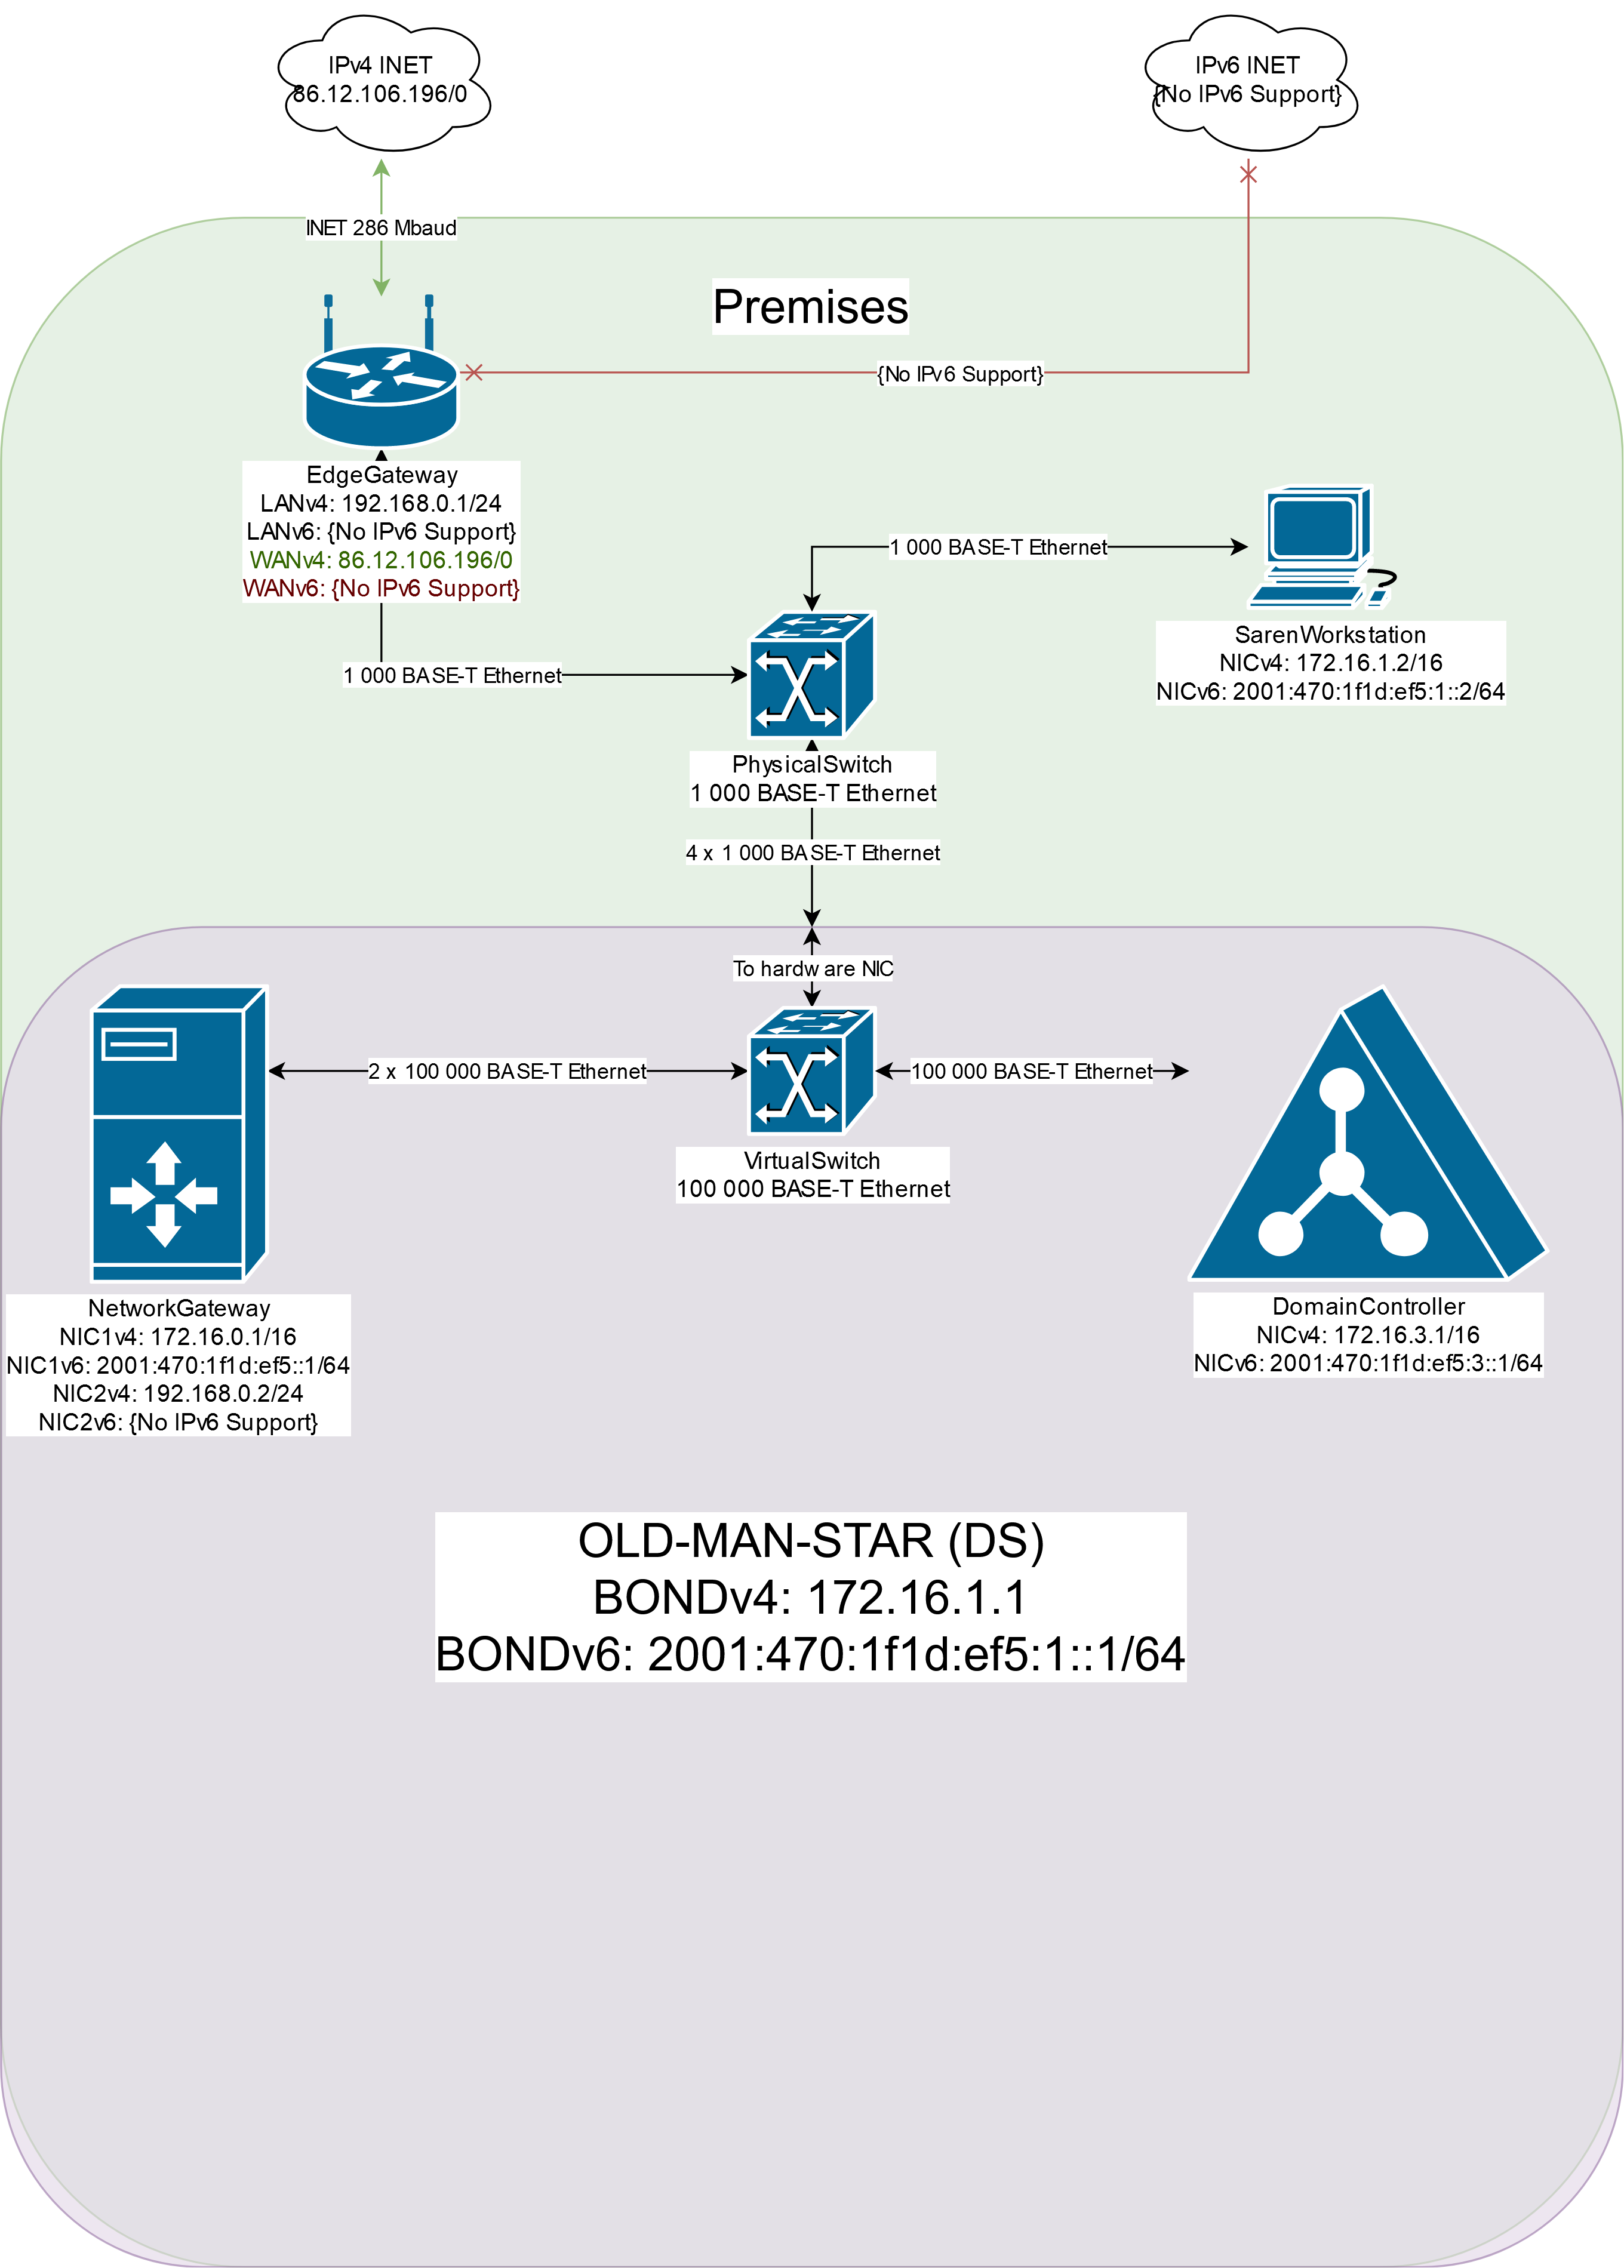
\includegraphics[width=\linewidth]{CITY3111/bitmaps/figure_3.png}
    \caption{A topology diagram of my pre-existing network configuration including DS inner workings}
    \label{figure_3}
\end{figure}

Working from the top down, I first believe the Internet needs no in-depth explanation. There are currently two versions of the Internet running in parallel: the older Internet Protocol (IP) version 4 (specified in RFC 791 \cite{ietf_1981}) which we all use on a daily basis to communicate, fetch data, share the general stuff we do, whoever we are and whatever we value. The second version of the Internet is the IPv6 suite (specified in RFC 8200 \cite{ietf_2017}) which is much newer, smaller and is not cross-compatible with IPv4. This suite was published to help ease a predicted squeeze on the address space found in IPv4.

My ISP does not currently feature IPv6 support, however my network does. This will be an important consideration in the design process I am about to undertake, as I will need to take extra care in ensuring that my guest OSes are capable of downloading packages and updates via the Internet and having a pre-configured IPv6 network may cause newer OSes to think there is an IPv6 gateway available when there isn't.

Moving downwards toward the on-premise equipment, I have three separate network devices outside of the DS: the edge gateway device, the physical switch and my personal computer Saren. Firstly, the edge gateway manages communications between all internal devices and the internet with a LAN subnet of 192.168.0.0/24. The physical switch operates on layer 2 of the OSI model \cite{day_et_al_1983} and facilitates communications between any physical devices on my network not connecting via the edge gateway's built-in Wi-Fi access point.

Next, my PC, Saren, will be used to oversee operations and issue commands to both the physical hardware on my network and the virtualised components found on my DS. I will achieve this by using a combination of the Proxmox VE web interface to manage the virtual hardware, Virt-Viewer to directly interact with the console of each individual guest OS and SSH to access teletype sessions on each system once they are fully configured.

Finally reaching the DS itself, this is where the nuts and bolts of the operation come into life. Within the DS there is another, much faster virtual switch which is used to virtually connect all of my guest OSes together. This virtual switch also has direct access to the physical NICs on the server to facilitate external communications.

In addition to the virtual switch, there are currently a plethora of guest OSes running various components of my home network. I have decided to include the two most vital ones however, and the ones that must run in order to provision a skeleton network (i.e. one with internet).

The Network Gateway operates as a communicator between the edge gateway and the rest of the network, providing a larger subnet of 172.16.0.0/16. It also acts as the only DHCP and DNS server advertised within my home network and provides DNS forwarding and caching to facilitate fast internet access for devices trying to access the internet.

The Domain Controller manages network-wide authentication tasks as well as timekeeping and policy-setting. The Domain Controller won't necessarily be of particular use to us however it does offer DNS propagation for internal network devices so it cannot be shut down during even the most minimal network environments.

\textbf{\sffamily{The existing network topology: Some examples}}

To demonstrate how devices currently connect to my network communicate, I will express some fictitious examples of communication routes. This is relevant simply because it helps build a picture in you, the reader's mind of the basic structure involved in this system.

First, lets imagine Saren wants to acquire some arbitrary data from a session-less (i.e. UDP) source on the internet. Without diving into the differences between the TCP and UDP protocols, Saren would send a request which would first travel to the network gateway via the physical and virtual switches. The network gateway would then recognise the destination of the request as external and send the packet to the edge gateway via the virtual and physical switches once more. The edge gateway will then send the request off onto the internet, and from there direct and responses via the same path the request was sent (i.e. to Saren via the network gateway).

I appreciate how complex such an example may be, so allow me to explain another, perhaps simpler to grasp example to supplement my main paragraph above. Imagine again some session-less request happening, but this time it is being done by the hypervisor itself, Old-Man-Star. As the hypervisor is technically also hosting the network router, any data exchanges all happen internally across the system busses. The resultant computation is a request packet destined for the edge router and ultimately the internet, which will go via the physical router. When viewed in this sense, one of the potential advantages of using a hypervisor to prototype OpenMPI software becomes apparent: there is a huge drop in the delay experienced when exchanging information that would otherwise need to travel between two physical nodes.

\textbf{\sffamily{The revised network topology: The five guest OSes \& other alterations}}

Armed with a topology map and a detailed understanding of the network structure as a whole, I can now explain to you the additions I will be making to the structure of the network and why.

As displayed in the revised topology map, I have decided to add another virtual switch into my DS's hypervisor. The logic behind this thought process is that by separating the MPI nodes onto their own switch with a dedicated IPv4 and IPv6 subnet, I can avoid regular network traffic. This solves issues that were discussed previously regarding bandwidth contention and also avoids or even negates entirely the likelihood of packet clashing.

Aside from the addition of a second virtual switch, the only other addition is the guest machines themselves. The guests are connected to both the existing virtual switch and the new, dedicated virtual switch over two 100 000 BASE-T Ethernet NICs per node. This is essentially the only major changes made to the network configuration, my philosophy being that by keeping the network fundamentally unchanged where it isn't necessary will help retain the pre-existing stability as best as possible.
\vfill\break

\begin{figure}[H]
    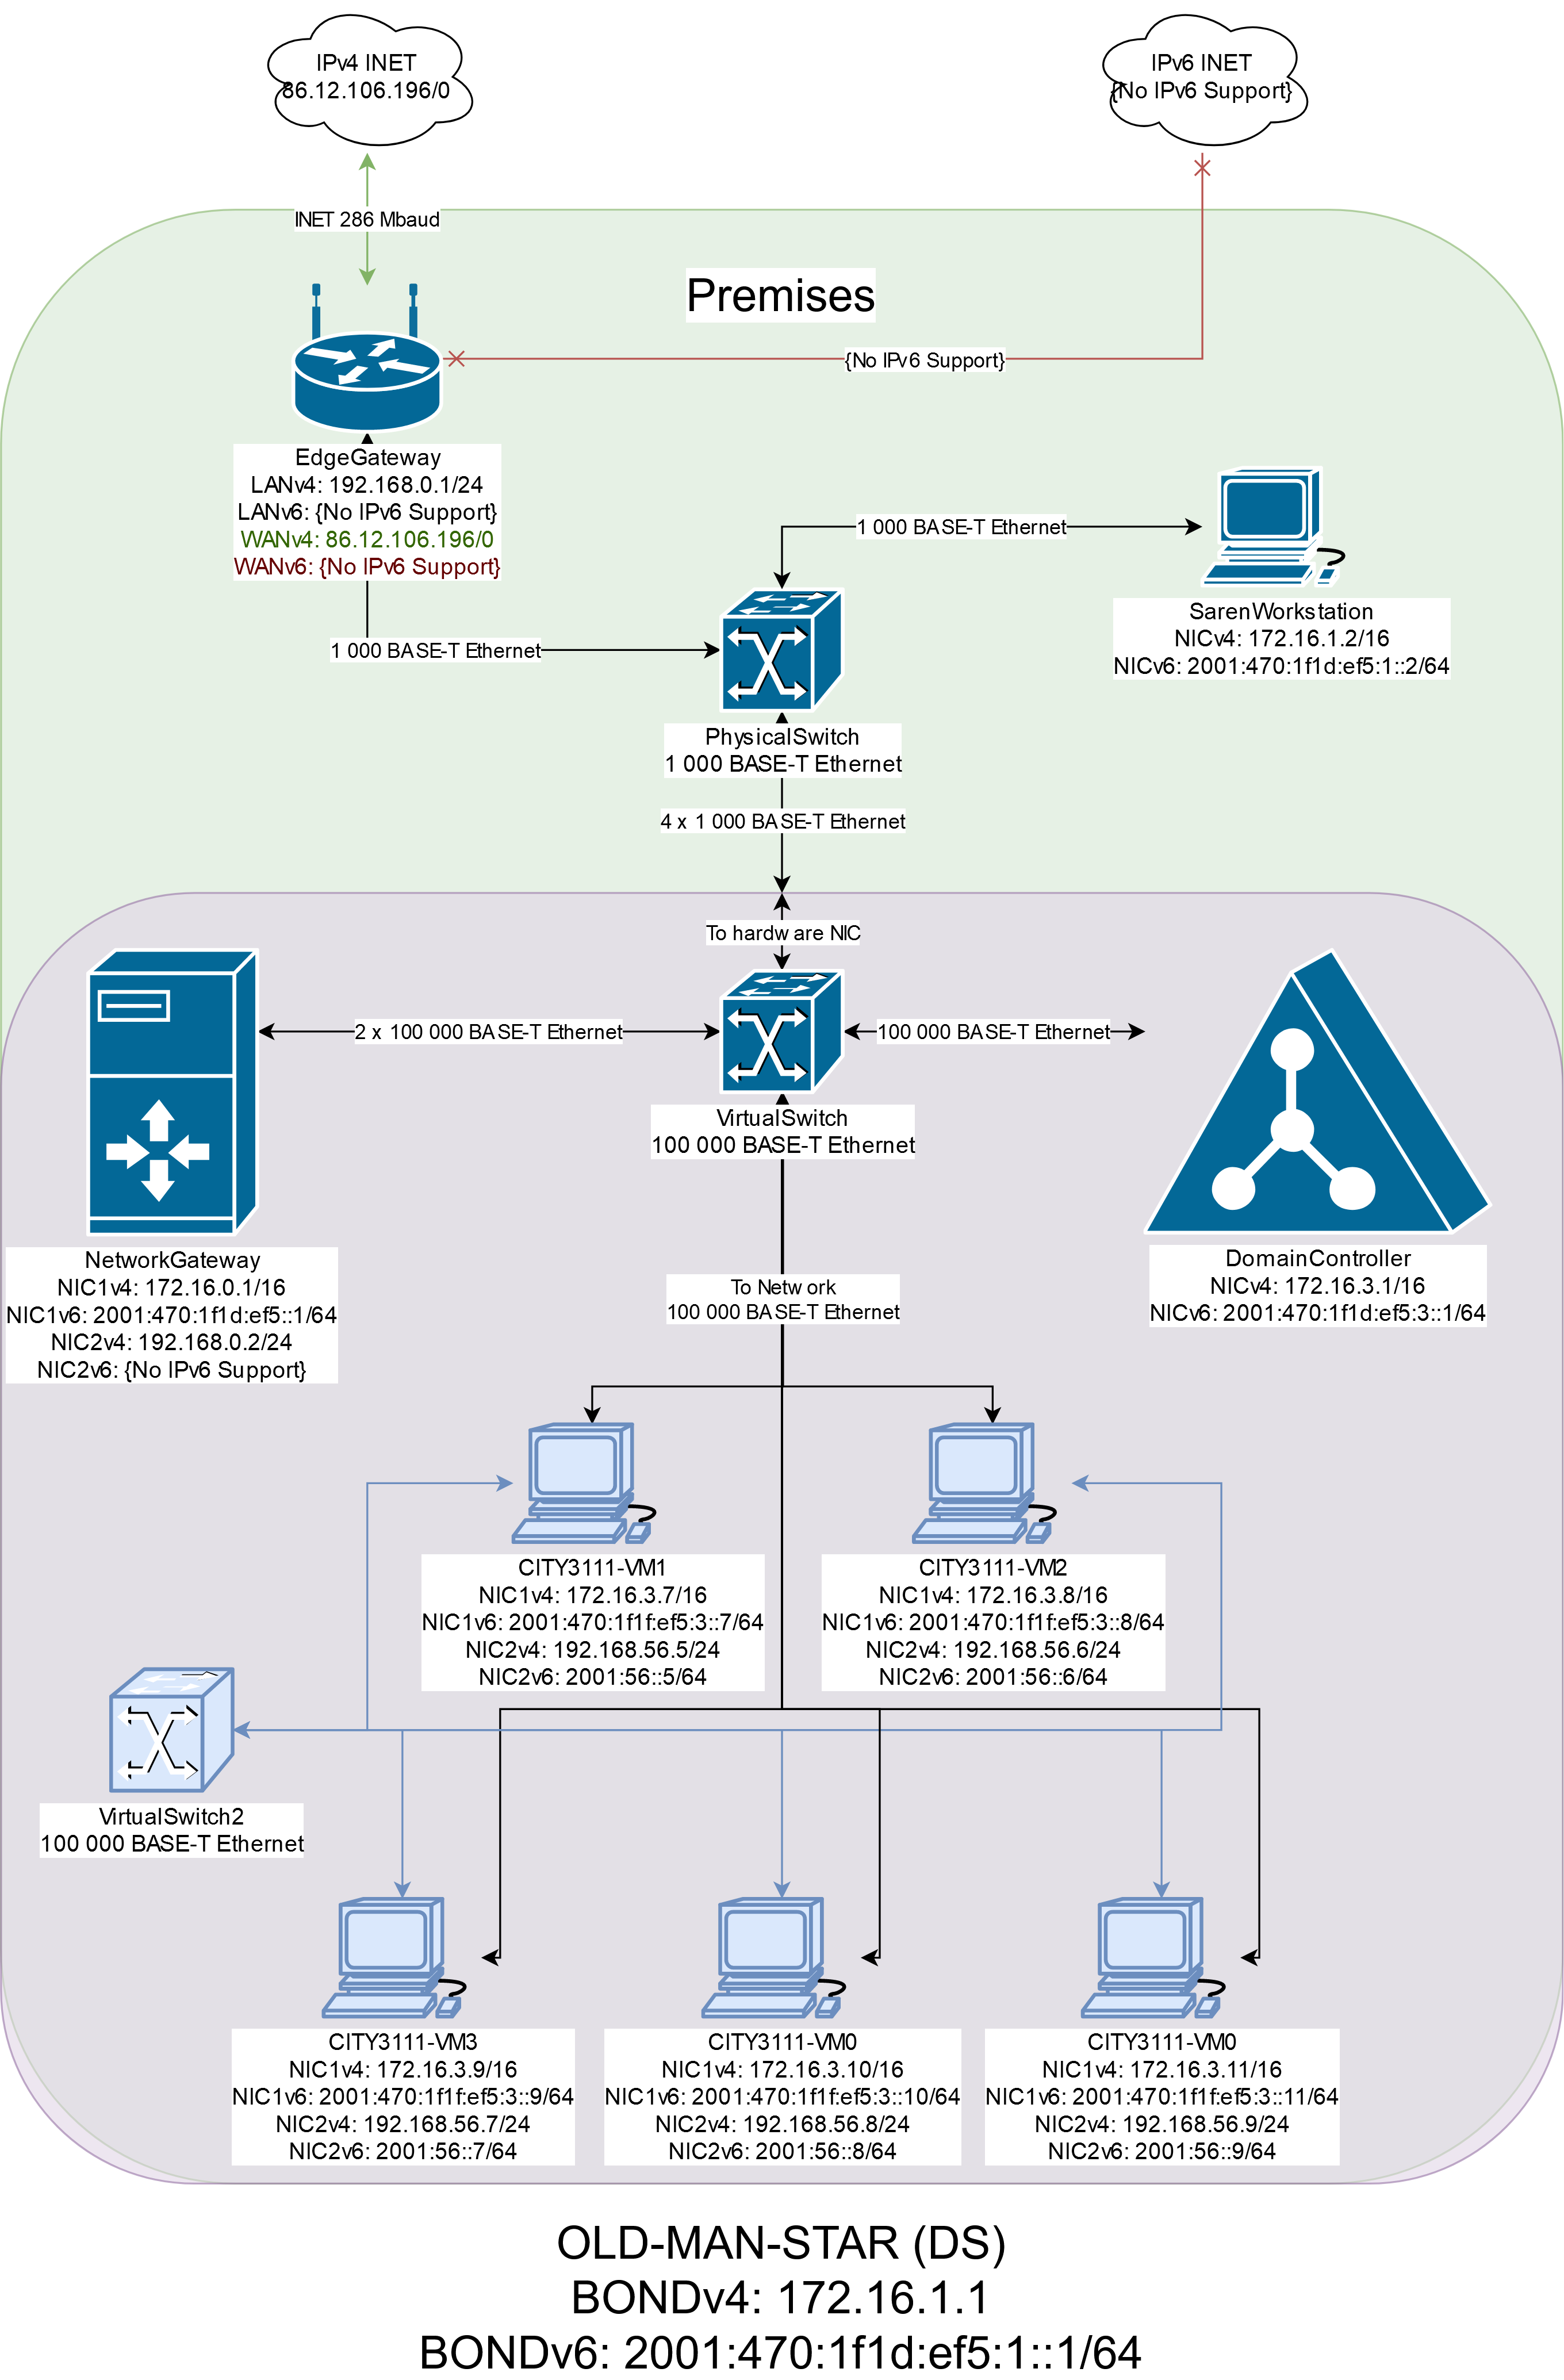
\includegraphics[width=\linewidth]{CITY3111/bitmaps/figure_4.png}
    \caption{A topology diagram of my revised network configuration including a second virtual switch}
    \label{figure_4}
\end{figure}

\section{Designing my cluster: The software design \& configurations}
Hardware design complete, my next stage is to design the software. Software used in my project can be divided up into two subcategories: packaged software and custom software.

In this document, the term packaged software expands to cover all software not written by myself, which includes the operating systems in use throughout the cluster in addition so any software running on them. Custom software will refer to any software I write to run atop OpenMPI.

\textbf{\sffamily{Designing my test environment: hypervisor re-configurations \& guest considerations}}

In order to have a place to install, compile, run or test software effectively I need the hypervisor to be configured correctly and optimally. Currently, large portions of my DS are configured for stability, which in some cases means utilising older firmware packages or opting for software solutions to handle certain virtualisation tasks.

While this is acceptable and even recommended in production environments, in development environments, the less hindrance to performance the better the end results in most cases. To best optimise my virtual Beowulf cluster, I will apply more experimental or hardware-centric virtualisation methods where possible to deliver the best possible results during testing.

\begin{figure}[H]
    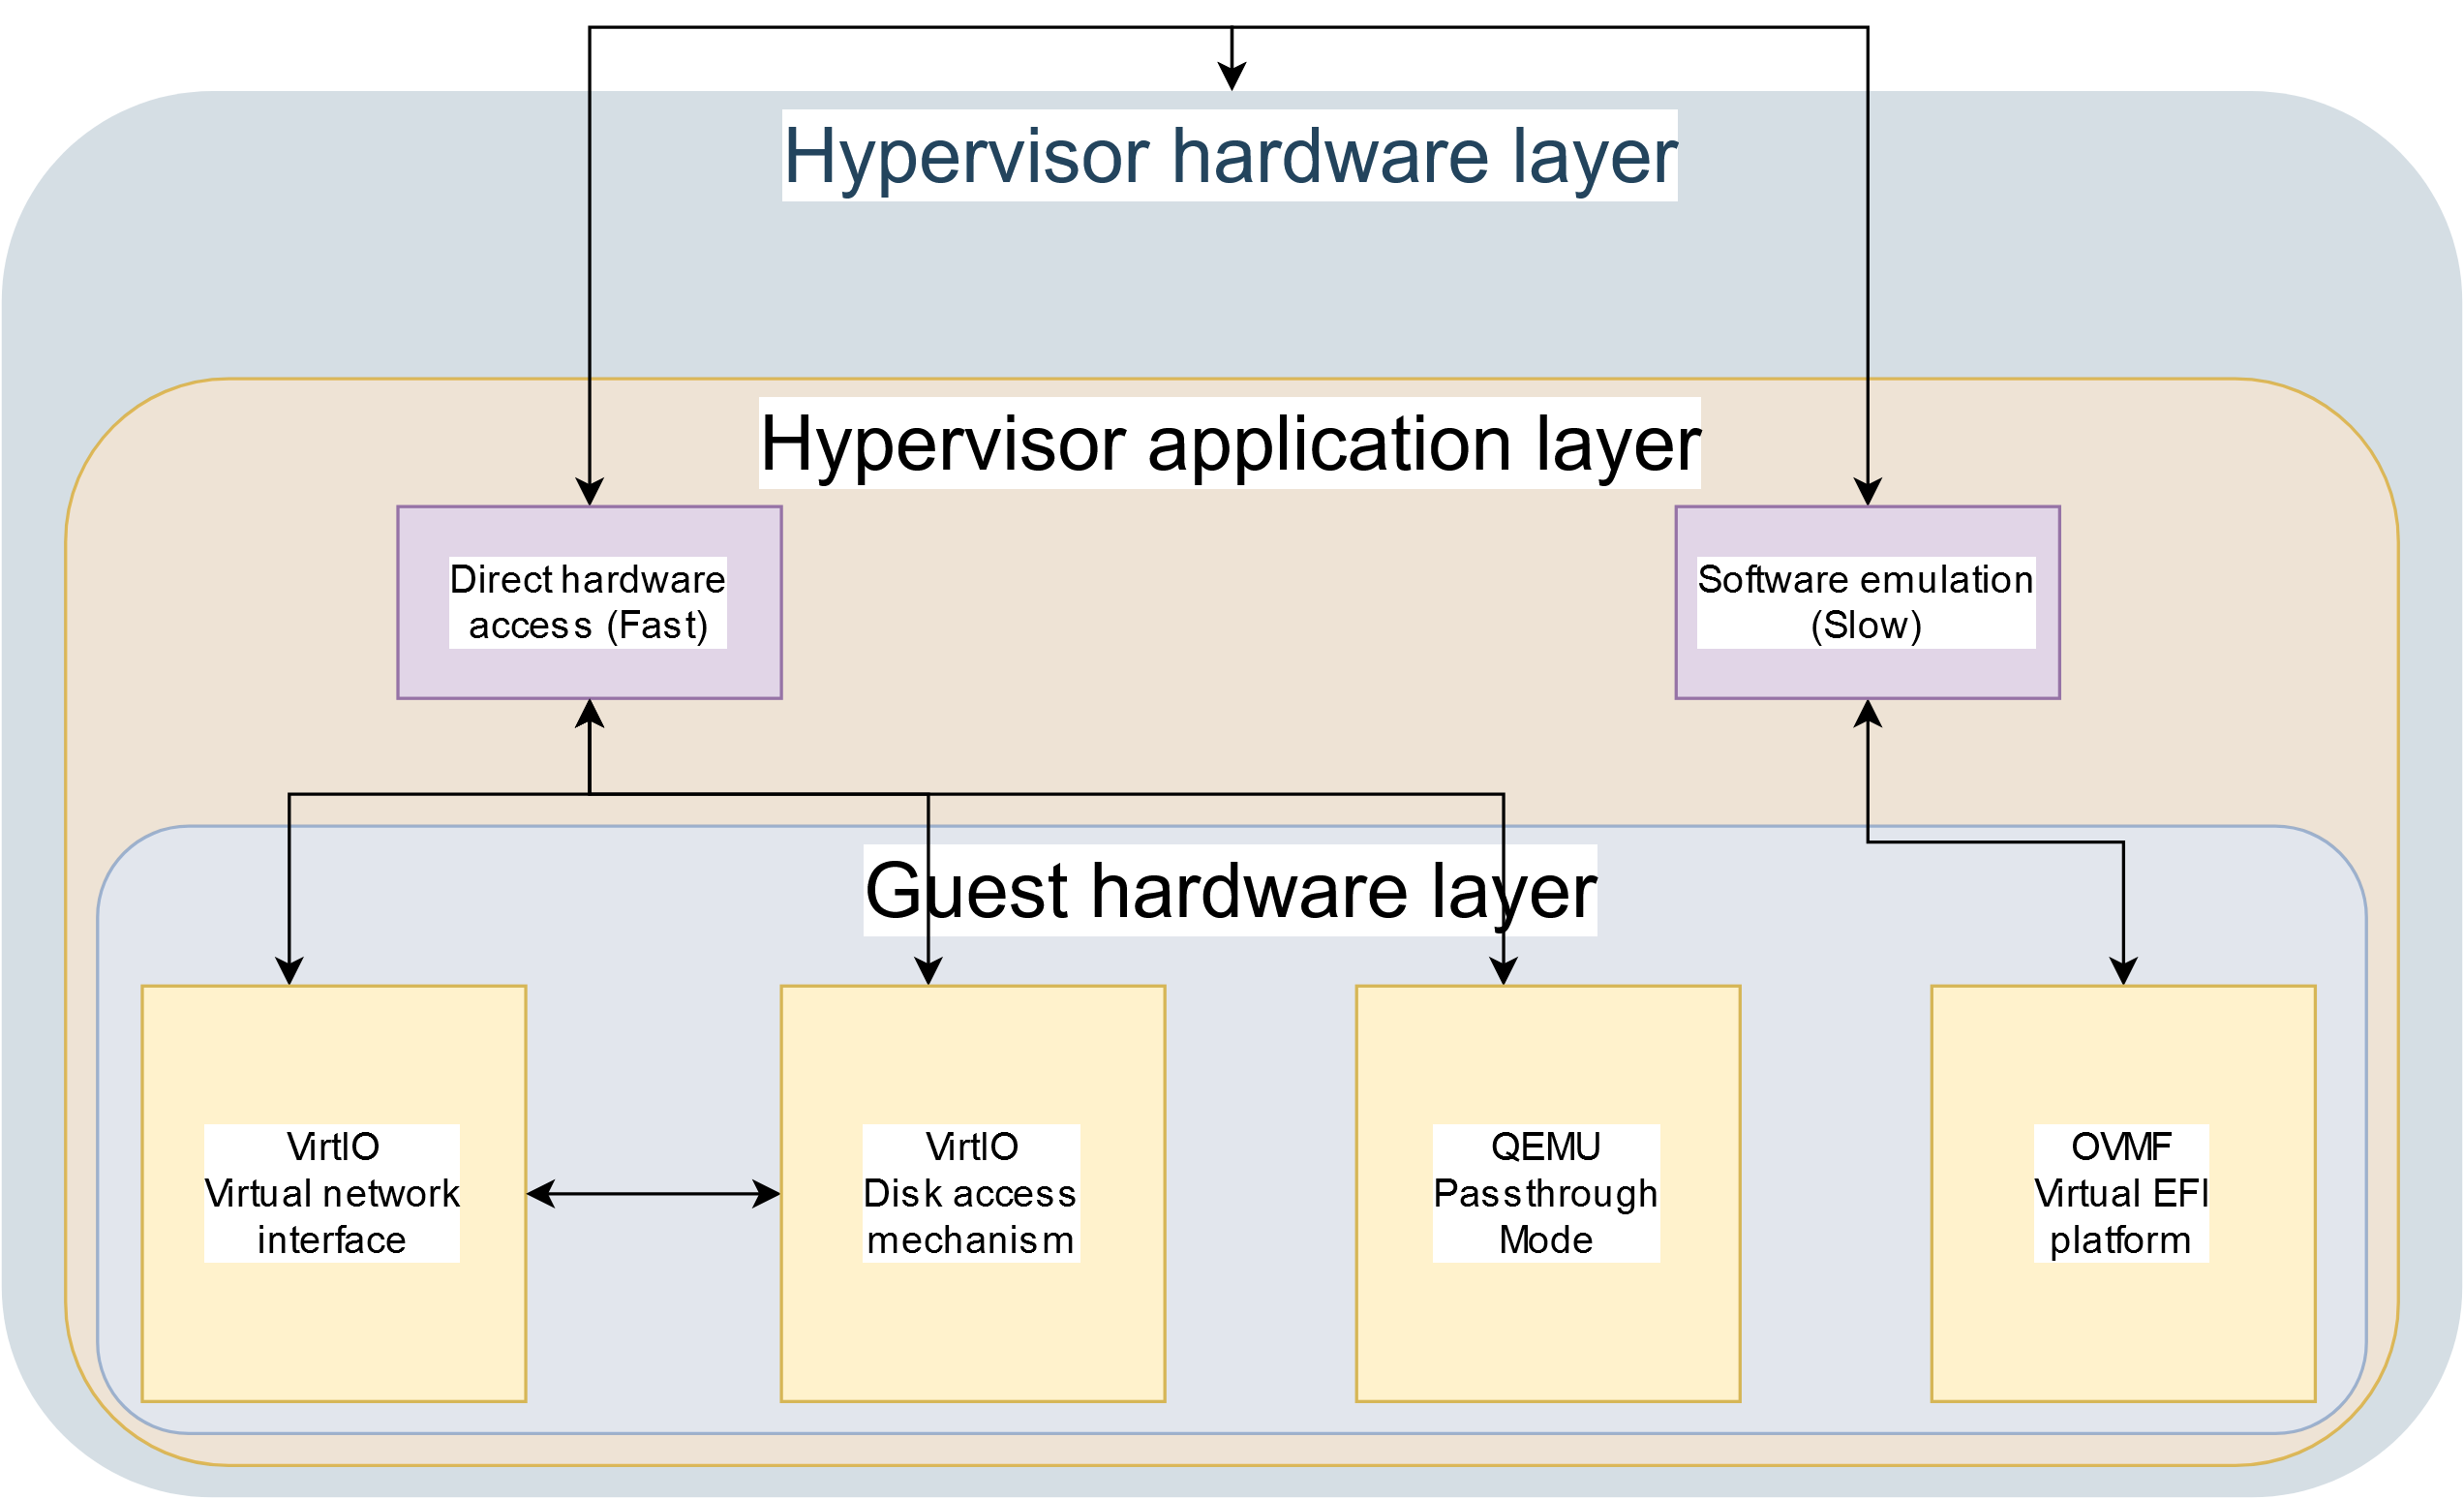
\includegraphics[width=\linewidth]{CITY3111/bitmaps/figure_5.png}
    \caption{A general overview of my hypervisor architecture design}
    \label{figure_5}
\end{figure}

My hypervisor uses KVM/Qemu for virtualisation which means it is incredibly diverse and can even emulate other CPUs and CPU architectures. While this can and, indeed, has been a feature of great usefulness to me outside of this project, it is also a potential barrier to optimal performance within this task.

The solution offered by Qemu, as seen in the figure above, is passthrough mode. By enabling this flag, Qemu will avoid emulating different CPU architectures or instruction set extensions and will instead offer the full suite of hardware CPU extensions to the virtual machine with its original model number and architecture in tact. This is the fastest available CPU model within the Qemu virtualisation software as there is virtually no software interference from Qemu/KVM during code execution. I will pass through a single core per node from each socket, offering load-balancing across both CPUs to minimise overall time requirements on the processors.

In addition to making changes to the way CPUs are presented to the guest machines, I will also be ensuring the mechanisms used for other virtual hardware components have minimal software overhead on the hypervisor. For example, Qemu/KVM offers a suite of firmware packages collectively known as the VirtIO drivers \cite{ova_2020} which permit closer access to physical hardware from within the virtual guest.

I will apply the VirtIO device types to my network adapter and virtual disk I/O bus. This should offer me maximum bandwidth between the virtual machines as well as between the virtual machines themselves and the DS RAID array. VirtIO is the only virtual network adapter type within Qemu/KVM that allows for 100 000 BASE-T Ethernet speeds.

As the system has 96GB of RAM available, I will present the full 4GB of RAM found on the reference hardware, the Raspberry Pi. While software requirements should not exceed that figure per node, it is a trivial task to allocate more memory to the virtual guests if it is so required.

Lastly, I will also opt to use an EFI bootloader over a virtualised BIOS. While this is less relevant to performance as a whole, I still felt it was worth mentioning at the end of this subsection due to the impact it may play when hardware requests are made by a guest machine.

EFIs hands more device access over to the operating system in the early stages of booting which means that they start up faster and have the ability to call directly on hardware with greater ease. While this is unlikely to make a resounding difference it at all to my test program, it could help and enabling it will do no harm otherwise.
\vfill\break

\textbf{\sffamily{Designing my test environment: A breakdown of the guest software architecture}}

With the hypervisor configuration and architecture design complete, the next stage is to design my guests. Each guest will be as close as possible to a carbon copy of one-another, possible through last minute imaging of each machine from a preconfigured master.

The fundamental logic behind this is, if the differences between each node in the cluster are minimised, the test can be deemed as more scientific. The same background processes should run at start up, so the systems can be gauged as more alike at startup and during operation and the same firmware should be installed to the same version numbers.

\begin{figure}[H]
    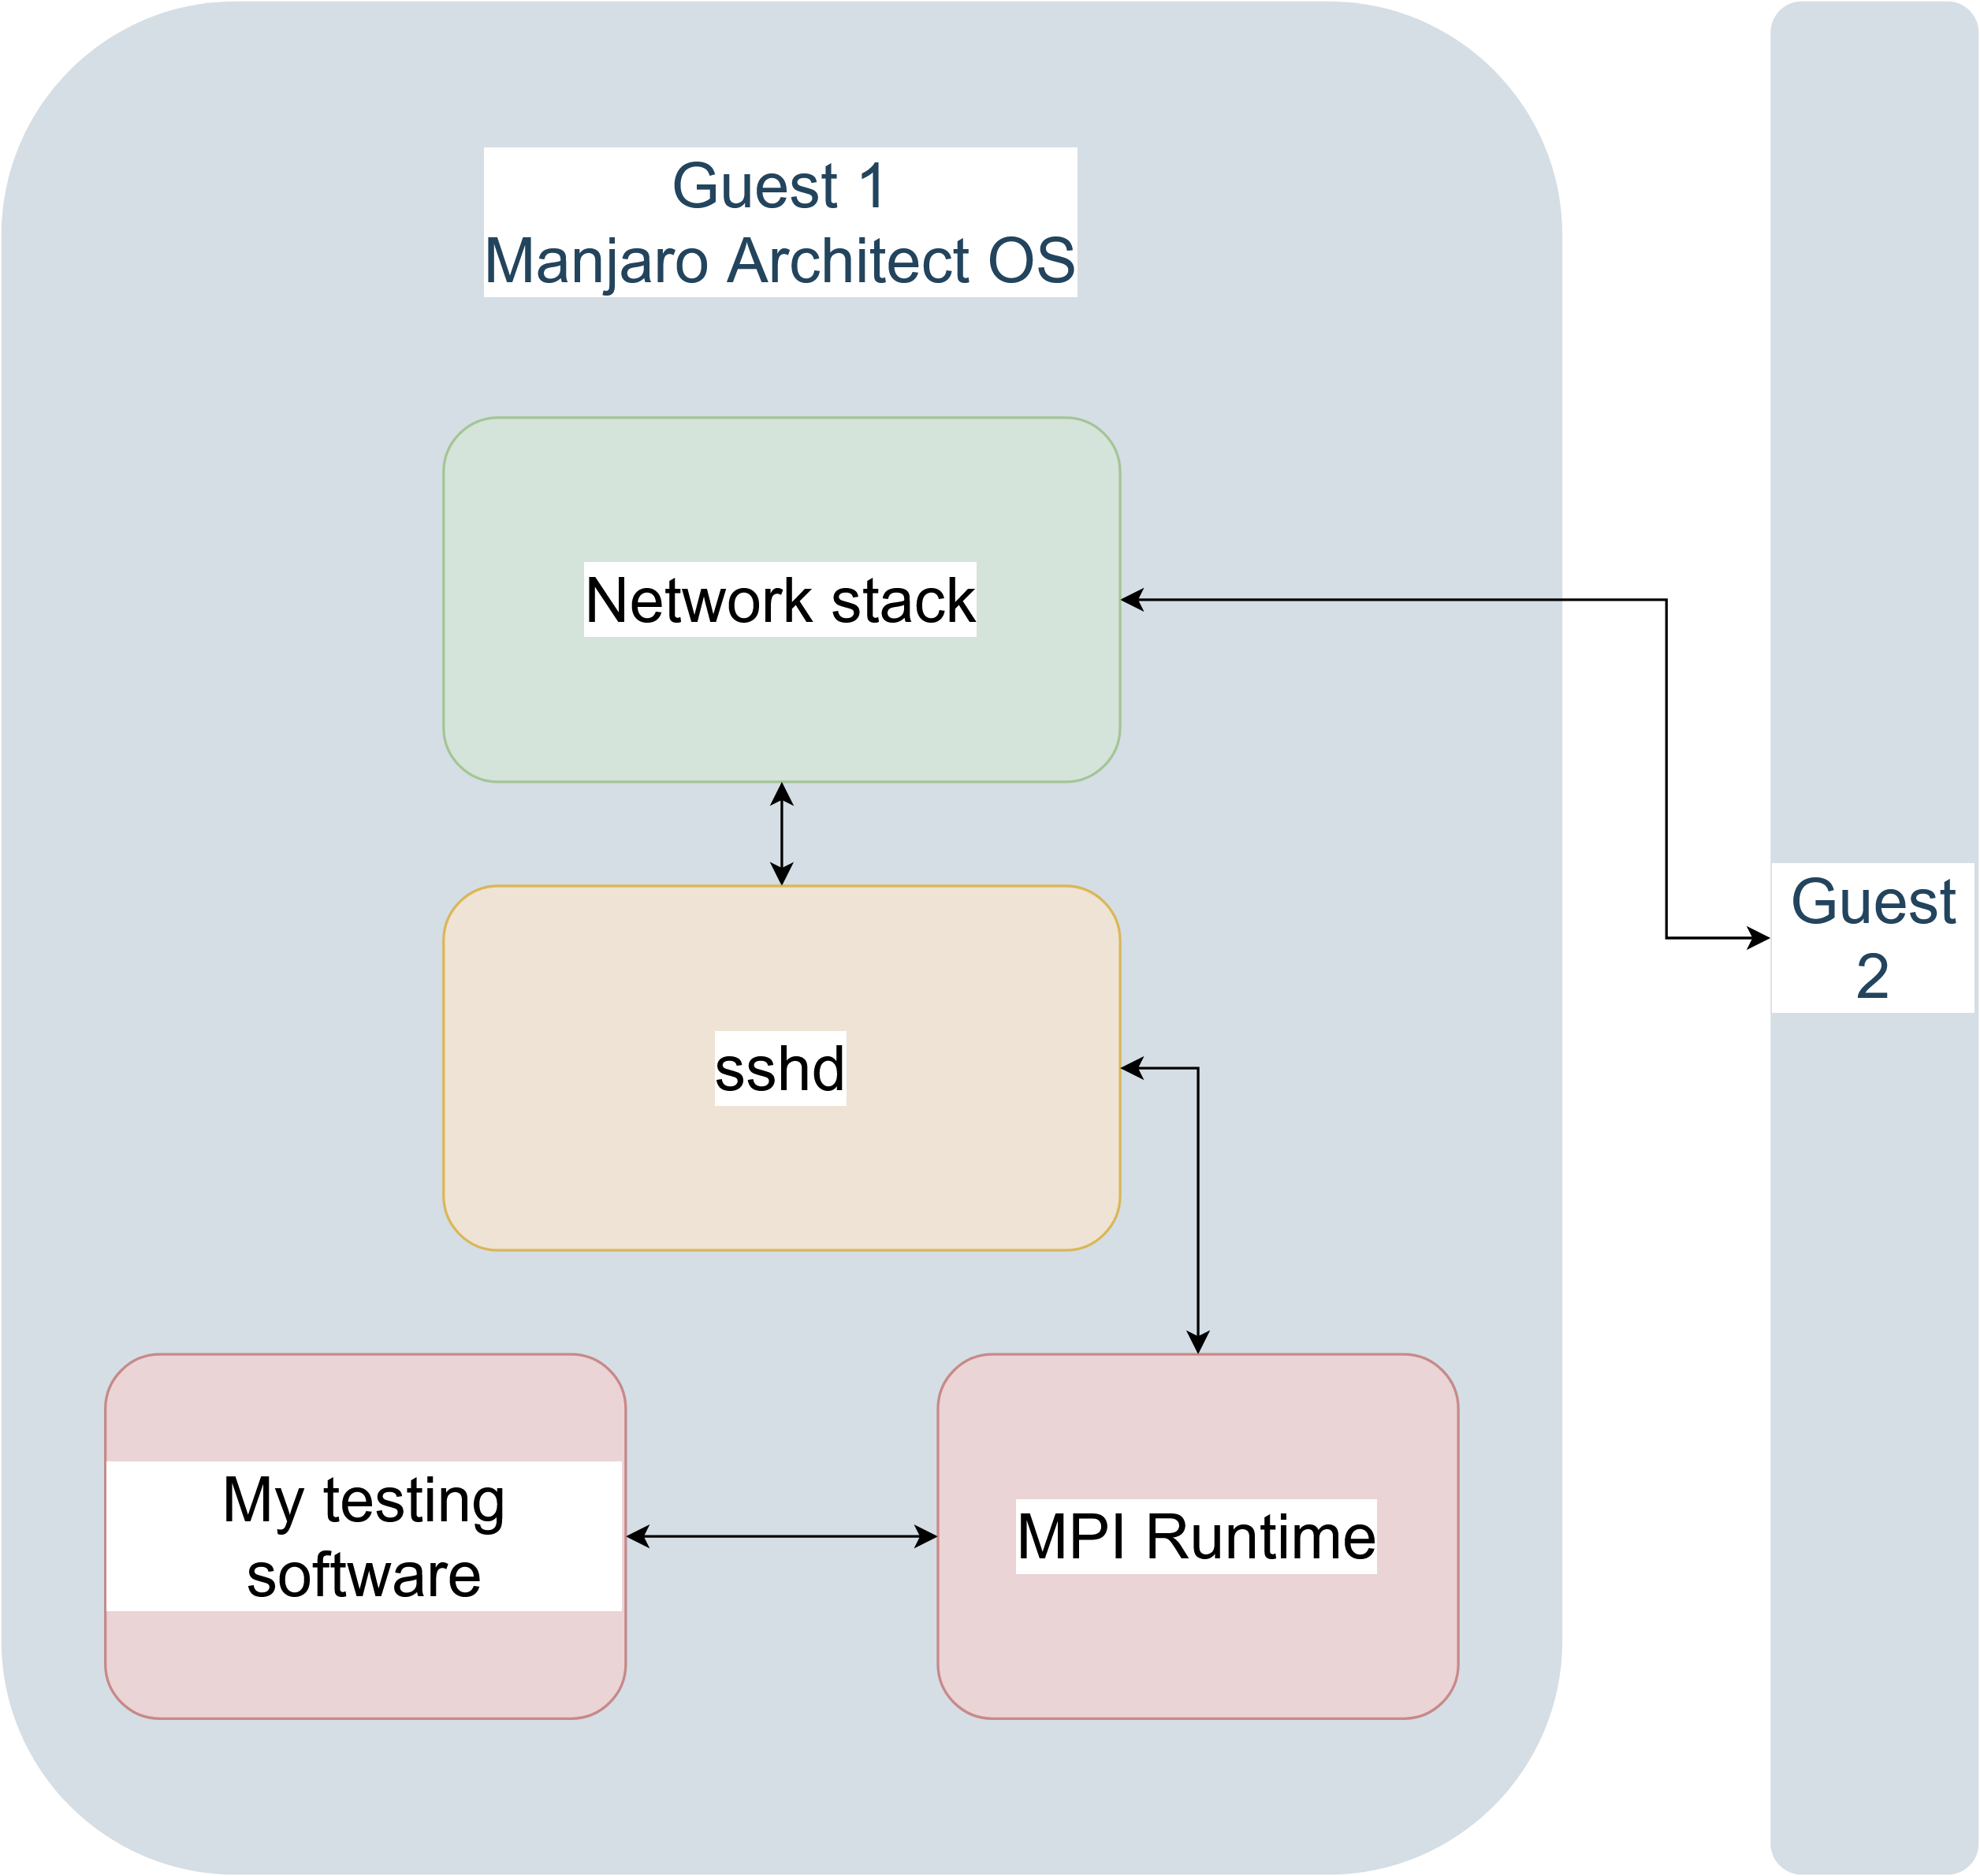
\includegraphics[width=\linewidth]{CITY3111/bitmaps/figure_6.png}
    \caption{A visual representation of my goal message-passing architecture}
    \label{figure_6}
\end{figure}

The main packages I will require have already been discussed in detail, but as a recap, they are the VirtIO network device firmware, OpenSSH and the MPI runtime. Each software package will need to interact with the others, as well as with the network device firmware. Ultimately, the network device firmware will be responsible for external communications with OpenSSH being the application layer for network transactions. The MPI runtime will thus act as a translator between OpenSSH and my own custom software.

With regards to my own custom software and how that communicates with the wider guest operating system, I will require the mpicc compiler (not noted in the diagram above) to compile the various hooks required by the runtime into my binary. Typically, the mpicc compiler is included in the same package as the runtime (in Arch's case, openmpi).

\section{Building my custom software: A problem to test my multi-nodal network}
In order to test my system architecture thoroughly, I am in need of a problem which can be easily divided between processes with sufficient computational expense to raise each CPU thread to its maximum throughput. The problem should also be of peer-reviewed nature in that it should use a principle already widely explored and proofed already by an external, verifiable source.

In my research for a suitable problem, I discovered a few problems which might be suitable for stress testing my Beowulf cluster, but the two I will discuss here will be hashing functions and fitness optimisation functions. I will use this section to finalise this paragraph by discussing these two methods, why I've chosen one over the other and how I plan on implementing my chosen method.

\textbf{\sffamily{Two methods for testing my cluster: hash functions primer \& discussion}}

Cryptographic hash functions are defined as the mathematical algorithms which can `digitally verify' a data block. Specifically, it aims to create a string typically fixed in length which can uniquely represent a quantity of data such as a string, file, binary or file system.

The study of what we today understand as hash functions began in the 1970s with the Diffie-Hellman (DH) method \cite{diffie_et_al_1976} which underpins modern public/private cryptography methods used to exchange data over public transmission lines such as the Internet.  In short years, Rabin \cite{rabin_1979}, Merkle \cite{merkle_1979} and Yuval \cite{yuval_1979} (amongst others) quickly built upon the DH model, offering real-world applications to the public key cryptography concept that today drives secure communications everywhere.

Between the 1970s and 1990s cryptography of this kind did not see particularly wide mainstream adoption outside of specialist computing and it wasn't until the late 1990s and the major adoption of the Internet as a common data exchanging environment that caused an upsurge of DH-modelled algorithms to emerge and gain widespread usage for general cybersecurity purposes. \cite{preneel_2010}

Modern hash algorithms such as the SHA-2/SHA-3 suites and EdDSA still base themselves on the original DH paradigm, where the fundamental changes are less structural and more mathematical in nature. Due to the increasing mathematical complexity required to secure systems that get faster over time, calculating hash functions using a sufficiently modern algorithm against a sufficiently large block of data should result in high CPU load for a long enough time-frame to get a strong data-set with which I can scientifically analyse.

Hashing functions can therefore be seen as one potential method of benchmarking a cluster, especially when one considers how susceptible many hashing algorithms are to parallelism. However, hashing functions are notoriously difficult to write so I would more likely than not need to find and utilise source code to compile my own hashing binary which is compatible with the MPI runtime. This would in turn require me modifying existing source code to contain MPI hooks and functions.

For the context of this degree-level dissertation, I think that a hashing function would likely incur too much complexity to be completed within a reasonable time-frame. I am therefore going to review my options and look down a different avenue of research.
\vfill\break

\textbf{\sffamily{Two methods for testing my cluster: fitness optimisation functions primer \& discussion}}

Fitness optimisation functions are ubiquitous in genetic programming as a way of testing how good a specific algorithm is at locating an optimal solution. Numerous fitness functions exist, however the most popular include the Rastrigin function, Ackley function, Rosenbrock function, Himmelblau's function and Eggholder function.

The main goal of fitness optimisation functions is to benchmark a genetic algorithm's performance against either other similar methods or improvements on an existing method. Every individual fitness function therefore has a different design and purpose in mind and offers different search-space constraints and granularity. To understand how fitness optimisation functions work, I will look briefly into two different methods, namely the Ackley and Eggholder functions.

The Ackley function \cite{ackley_1987} is a two-dimensional optimisation first conceived by David Ackley in 1987. It has a search space ranging between -5 and 5 and a global minima at \{ 0,0 \}. When visibly rendered on a three-dimensional plot, it assumes a funnel-like shape with peaks and troughs lining the fabric of the search space leading towards the centre of the grid.

\begin{figure}[H]
    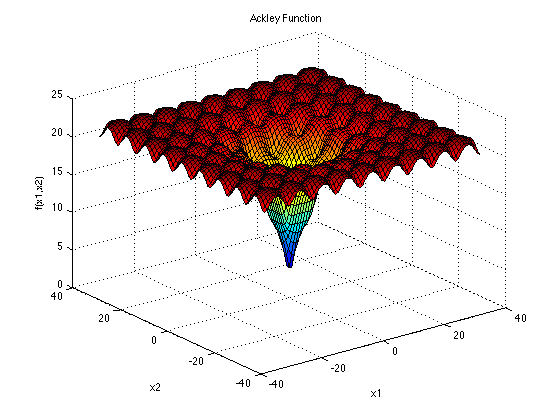
\includegraphics[width=\linewidth]{CITY3111/bitmaps/figure_7.png}
    \caption{A visual representation of the Ackley function \cite{surjanovic_2017}}
    \label{figure_7}
\end{figure}
\vfill\break

It is these peaks and troughs optimisation algorithms come unstuck with and it is precisely this characteristic that mathematicians hunt for in their efforts to form fitness functions. In the case of my software, in order to maximise results I hope to do the opposite of optimisation and actually add computational expense to the software rather than reduce it.

I will now take a brief look into a different function, the Eggholder.

The Eggholder function aims to fulfil fundamentally the same niche as Ackley's function did by providing a search space that contains a high volume of local minima in a comparatively small search space. In the case of the Eggholder, its search space is much larger than Ackley's with bounds between -512 and 512 with a general optima of -959{,}6407 at \{512, 404.2319\}.

\begin{figure}[H]
    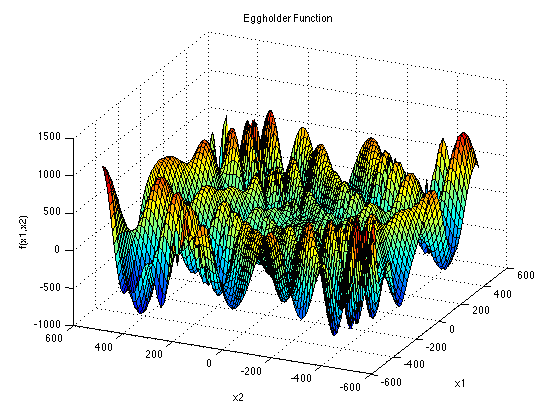
\includegraphics[width=\linewidth]{CITY3111/bitmaps/figure_8.png}
    \caption{A visual representation of the Eggholder function \cite{surjanovic2_2017}}
    \label{figure_8}
\end{figure}

Visually, Eggholder takes on a much wilder appearance than Ackley's function does. This makes it a lot tougher on optimisation techniques due to the heightened probability of getting trapped. While this doesn't necessarily convert to higher computational expense under my requirements, it does offer a larger search space which should provide deeper problem precision for me to exploit.

Unfortunately, despite heavy research, I have been unable to discover the origins of the Eggholder function. All my information, including the equation and visual models have to therefore come from Vanaret's work at the Université de Toulouse \cite{vanaret_2015}.

To test my cluster, I will be utilising the Eggholder function. I intend on searching the full search-space at all times, introducing nodes one by one to measure performance change as process counts increase. This will give me a suitable data-set with which I can scientifically analyse.

\textbf{\sffamily{Implementing a fitness optimisation function: My intended plan of attack}}

In order to create a piece of software which satisfies all the requirements while using the Eggholder function, I need to design with brute forcing in mind. In short, brute-forcing a fitness optimisation function differs from the function's intended purpose in that with an optimisation method one would aim to find the best optima as quickly as possible. In brute-forcing, the goal is to check every point on a grid given certain boundaries and precision values.

Eggholder allows for incredibly high precision (to confidently locate the global optima one would need to run approx. 26 214 400 000 000 calculations of the function's equation). If one was to take leverage of this function's complexity in conjunction with proper job division, a true parallel system in MPI could be achieved.

My plan in designing this system is to use a hybrid-master slave system on all nodes, rather than relying on job dividing and distribution using a centralised architecture. I believe using this design principle will simplify my codebase as well as speed up my cluster. If each node can compute its own problem bunch without external influence, bandwidth and computational expense is reduced.

If possible, MPI should only be responsible for two tasks. First and foremost, MPI should indeed be responsible for runtime management which includes process spawning and communications (`world management'). Secondly, MPI should facilitate the passing of results and only results from all nodes back to the parent (i.e. node 0). It is also worth noting that the combining of results from child nodes should be the only time the parent node is seen as the master.

\begin{figure}[H]
    \centering
    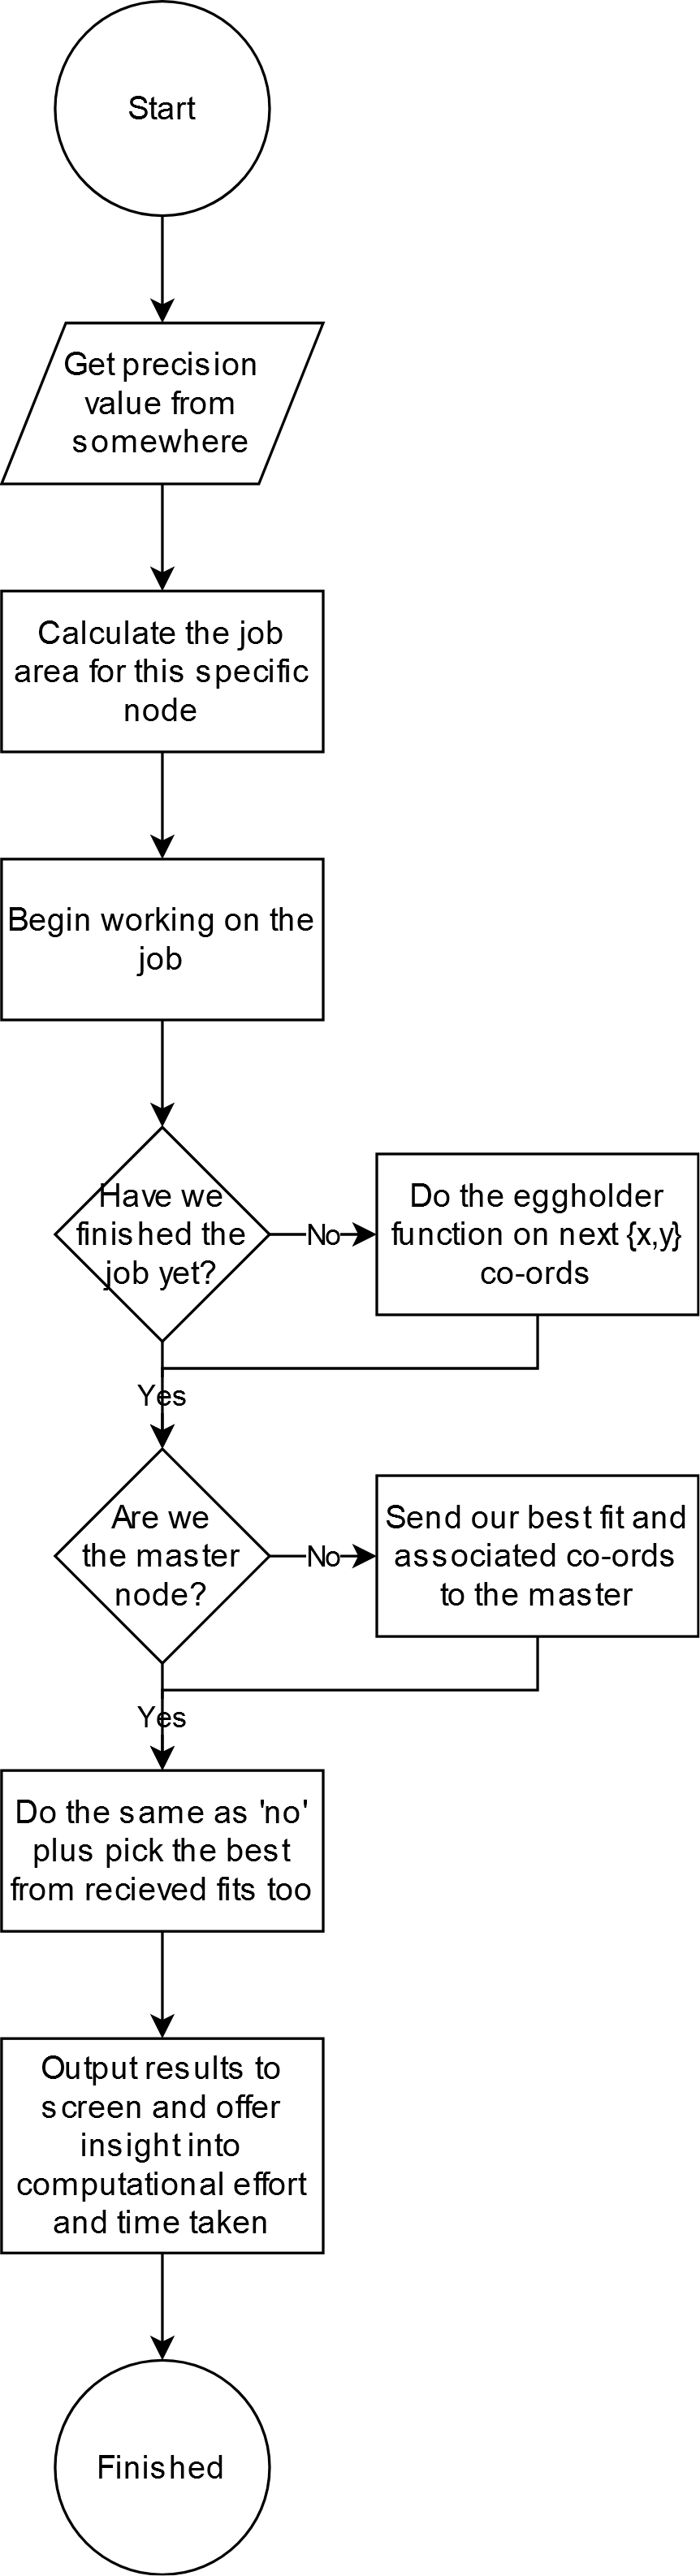
\includegraphics[width=55mm]{CITY3111/bitmaps/figure_9.png}
    \caption{UML diagram of my intended software architecture}
    \label{figure_9}
\end{figure}

As illustrated above, most of the process is handled internally by the individual processes. I hope that by utilising this design it is ensured that any reduction in speedups seen are purely based on hardware-induced granularity rather than avoidable network delays. Another feature worth noting in my design is message simplification by design. Rather than sending messages to the master every time a new best fit is found, each new best fit is stored in the node's own individual memory space. The best fit is sent back to the master at the end of the process before being compared against and stored or discarded depending on its quality comparable to prior results received.

The last two aspects of my design I intend on discussing are measurability and verbosity. Addressing the former first, I intend on measuring only one metric, that being time taken to complete the job. This can be achieved using a chrono clock in C++, most likely placed immediately before and after the loop responsible for the brute force process. By measuring the time taken to complete the job on the master, I will hopefully get a suitably accurate representation of how the process speeds change across the cluster as job sizes shrink with each new node.

Addressing verbosity, I plan on presenting several information points to help measure the inner-workings of my program. These values are as follows: computational effort per node, approximate cluster effort, delta time for master node (as discussed), the best fit, the best fit location and the node which located the best fit.

Hopefully with this design I can achieve my goal set forth in Chapter One. In the following chapter, I will explain how I go about implementing this project, including a breakdown of the hardware setup, software installation, creation and testing as well as a discussion on any problems that arise.
